\section{Introduction}

Our evolving relationship with \textit{truth} in the age of artificial intelligence is increasingly shaped by modern Language Models (LMs) \cite{Brown2020, Chowdhery2022, Touvron2023}. Despite their remarkable fluency, these models can generate content that is factually incorrect or unfaithful to the input context while remaining highly confident --- a phenomenon commonly referred to as \textit{hallucination} \cite{ji_survey}. Such hallucinated outputs, which often appear coherent and convincing, pose serious challenges to the reliable and trustworthy deployment of LMs, particularly as these systems are integrated into real-world applications at scale \cite{zhang2023sirenssongaiocean, 10.1145/3531146.3533088, Huang_2025, maynez-etal-2020-faithfulness}.

Hallucinations manifest in different forms. \citet{Huang_2025} distinguish between \textit{faithfulness hallucinations}, where the output contradicts the provided source or context, and \textit{factuality hallucinations}, where the model generates information inconsistent with real-world facts. Prior work has attributed these failures to factors such as training data artifacts, model architectures, and inference strategies \cite{lee_deduplicating_2022, onoe_entity_2022, zheng_why_2023}. While the term ``hallucination'' itself is sometimes debated due to its anthropomorphic connotations \citep{halu_debate}, the underlying issue of unreliable generation remains a critical concern, motivating the development of effective hallucination detection methods.

\begin{figure*}[t!]
    \centering
    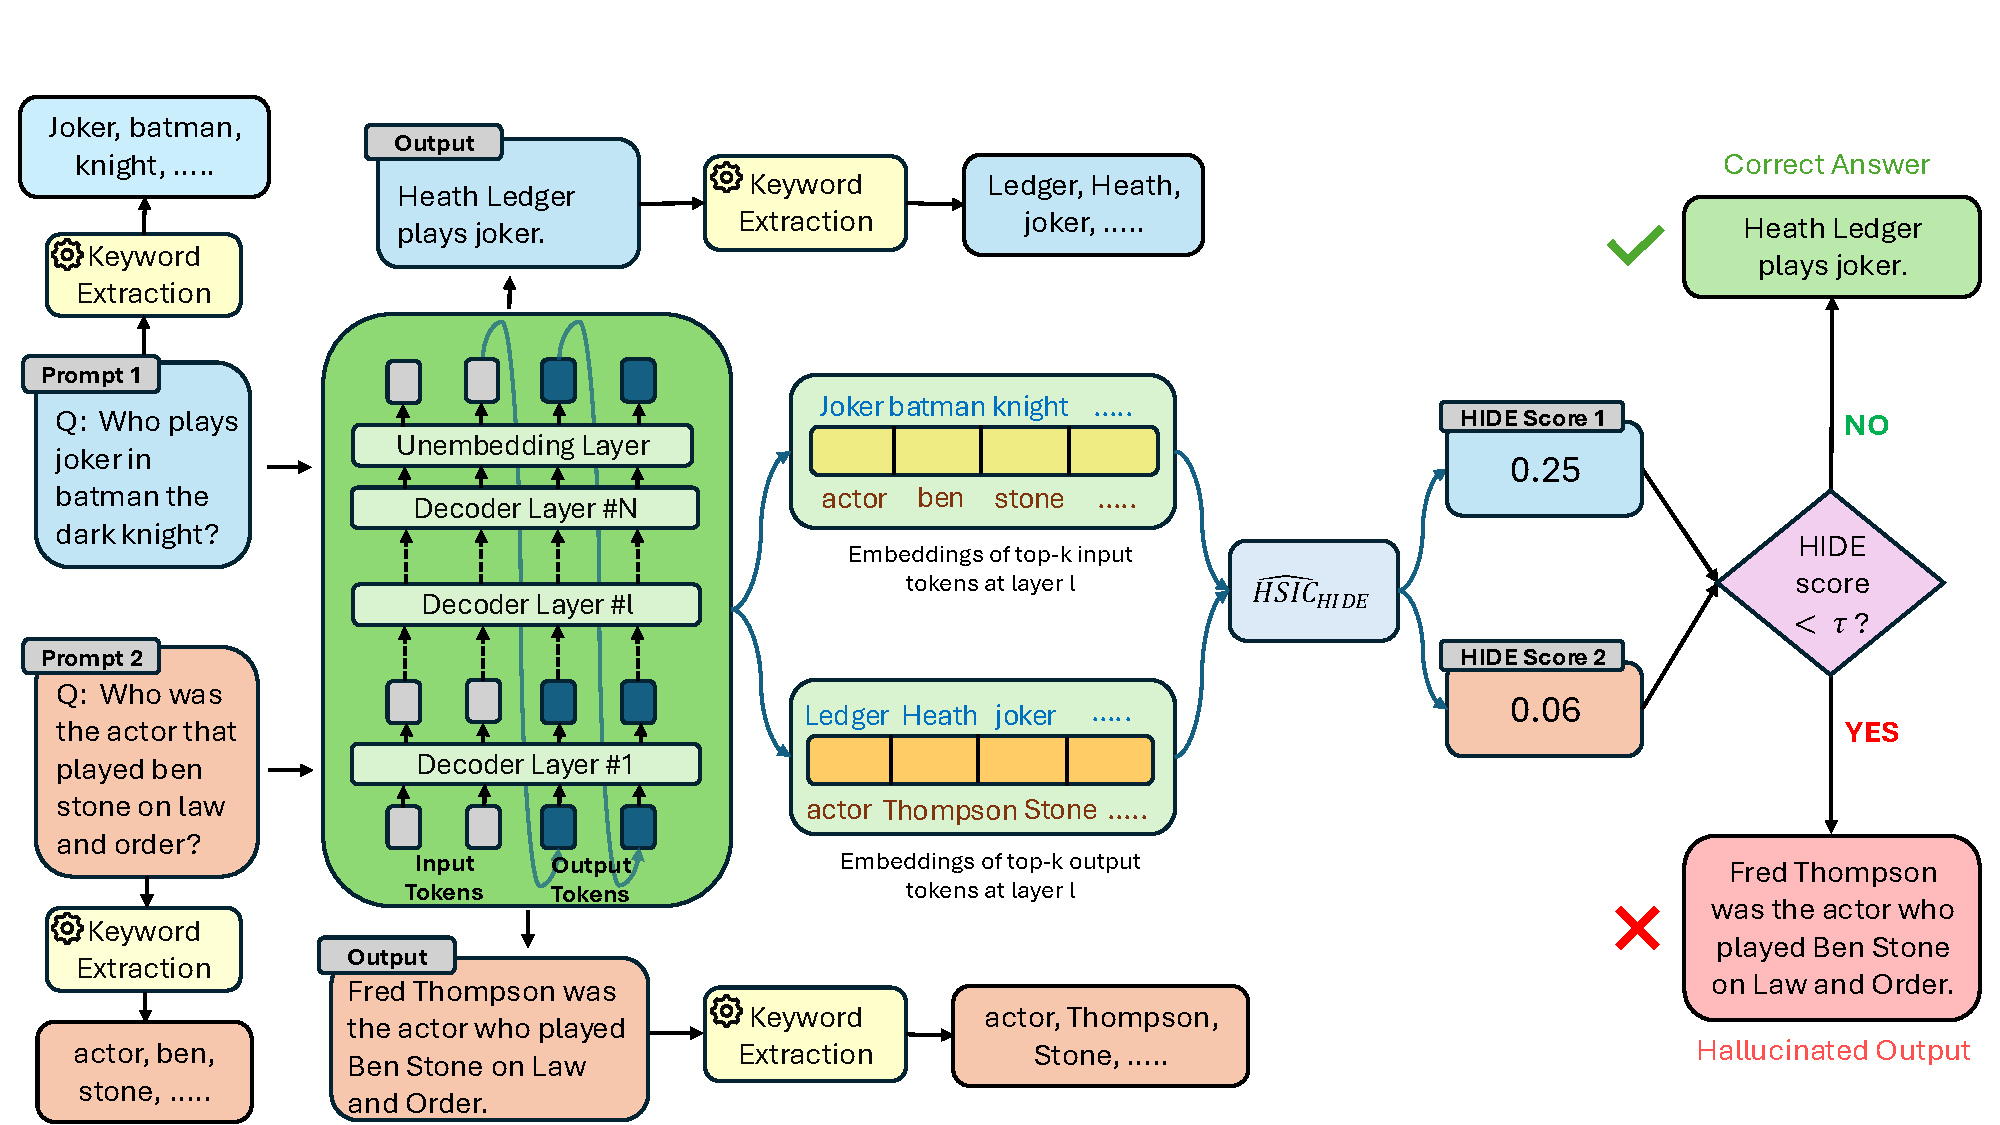
\includegraphics[width=\linewidth]{files/figures/hide.pdf}
    \caption{Our proposed method, \method, is a single-pass, training-free approach for hallucination detection. For a given input prompt, \method~extracts representative tokens from both the input and the LM-generated output, computes a \method~score using an adapted variant of unbiased HSIC on the corresponding hidden-state embeddings from a specific LM layer, and compares this score against a threshold to identify hallucinated generations.}
    \label{fig:intro}
\end{figure*}

A common approach to hallucination detection estimates model uncertainty using metrics such as perplexity \citep{ren_out--distribution_2023}, entropy \citep{malinin_uncertainty_2021}, or energy-based scores \citep{liu_energy-based_2020}, under the assumption that hallucinations correlate with low confidence. However, LMs are often confidently wrong, limiting the effectiveness of uncertainty-based signals \citep{simhi2025trustmeimwrong}. Another line of work detects hallucinations via consistency checks, generating multiple outputs per input and comparing them using lexical or semantic similarity measures \citep{lin_towards_2022, manakul2023selfcheckgptzeroresourceblackboxhallucination}. While effective, these approaches incur substantial computational overhead due to repeated auto-regressive decoding. Recent mechanistic studies further show that hallucination-related cues are encoded within LM hidden states \citep{azaria2023internalstatellmknows, ji-etal-2024-llm, duan2024llmsknowhallucinationempirical}, and some methods train probing classifiers on these representations. In contrast, our goal is to directly leverage internal representations for hallucination detection \emph{without} supervised training and \emph{without} requiring multiple generations.

To this end, we propose \textbf{\method} (\textbf{H}allucination Detect\textbf{I}on via \textbf{D}ecoupled R\textbf{E}presentations), \revisionr3{a training-free method motivated by the hypothesis that weaker dependence between input and output representations can indicate hallucination.} As illustrated in Figure~\ref{fig:intro}, \method~extracts hidden states corresponding to key tokens from both input and output sequences and applies an adapted variant of the Hilbert--Schmidt Independence Criterion (HSIC) to quantify representational coupling. \revisionr3{We test whether lower values of this adapted score help identify incorrect outputs.} \changedtwo{\revisionr3{Unlike multi-pass methods, \method~requires only a single auto-regressive generation per input, avoiding additional sampled responses; the resulting latency depends on the inference implementation.}}

\changed{We evaluate \method~on four question answering benchmarks --- SQuAD \citep{rajpurkar2016squad100000questionsmachine} and RACE \citep{lai-etal-2017-race} for faithfulness hallucinations, and Natural Questions \citep{kwiatkowski-etal-2019-natural} and TriviaQA \citep{joshi2017triviaqalargescaledistantly} for factuality hallucinations --- across six open-source LMs of varying scales and training paradigms, including base and instruction-tuned variants of Llama-3.2-3B, Llama-3-8B \citep{grattafiori2024llama3herdmodels}, and Gemma-2-9B \citep{gemmateam2024gemma2improvingopen}. These QA settings allow objective verification of hallucinations against reference answers; we additionally include dialogue experiments to assess generalization beyond QA.}

\revisionr3{Our main contributions are:}
\begin{itemize}[nosep, wide, labelwidth=!, labelindent=1.5pt]
\item \revisionr3{We introduce a training-free detector computed from selected hidden states during one generation, without attention-weight extraction, and evaluate it on faithfulness and closed-book factuality benchmarks.}
\item \revisionr3{We evaluate six models across four QA datasets, compare with a supervised probe, and examine dialogue, decoding, and other design choices. A direct comparison with attention mass and input-derived norm baselines shows where each detector performs well. A selected-token-count control helps assess what the HIDE score measures.}
\item \revisionr3{We measure a $50.8\%$ mean latency reduction relative to five-generation EigenScore under standard HuggingFace inference. Separate measurements of the overhead added to generation extend to Gemma-2-27B and show how it varies across models and datasets.}
\end{itemize}

\revisionr3{The ablations examine layer, kernel, and token-selection choices (\cref{sec:ablations}). We discuss these results alongside the attention and token-count comparisons to distinguish detection performance from evidence about the proposed mechanism.}
\changedtwo{\revisionr3{Together, these experiments show when HIDE is useful and where simpler signals perform as well or better.}}
